\documentclass[fr]{../../../../../../eplexam}
\usepackage{../../../../../../eplunits}
\usepackage{../../../../../../eplelec}
\sisetup{per-mode=symbol}

\DeclareSIUnit\tour{tr}

\hypertitle{Élecricité et Magnétisme}{2}{EPL}{1202}{2012}{Août}{All}
{Mattéo Couplet}
{Claude Oestges}[
    \paragraph{Remarques} 
    \begin{enumerate}
        \item \textbf{Ne faites pas confiance à ce document}. 
            Ce prétendu solutionnaire n'a été vérifié ni par des professeurs, 
            ni par des tuteurs compétents et peut donc contenir des erreurs. 
            Si vous en trouvez, ou si vous 
            avez une méthode plus rapide pour résoudre
            un exercice, n'hésitez pas à le signaler dans la 
            section \texttt{issues} du projet accessible par le lien ci-dessus.
        \item L'usage d'un formulaire récent (p. ex. 2015--2016) rend certaines
            questions triviales ; par conséquent, on considéra comme formules 
            acquises uniquement les lois fondamentales et les définitions.
    \end{enumerate}
]

% \begin{document}

\section{}
Un disque diélectrique circulaire de centre $O$, de rayon 
$a = \SI{10}{\centi\meter}$ et situé dans le plan $xOy$, 
porte une charge $Q = \SI{e-6}{\coulomb}$ répartie uniformément 
sur toute sa surface. 
Ce disque tourne à raison de \SI{3000}{\tour\per\minute} dans le sens positif 
(main droite autour de l'axe $Oz$).
Calculer le champ d'induction magnétique $B$ apparaissant au centre de ce 
disque. Pour le calcul on considérera ce disque comme un dispositif plan sans 
épaisseur.

\begin{solution}
    Pour résoudre le problème, nous allons diviser le disque en une série 
    d'anneaux concentriques. On peut tout d'abord affirmer
    \[ \B = \int \dif\B = \mu_0 \int \dif\H \]
    Aucune information sur la perméabilité relative n'est donnée ; on peut 
    donc admettre que le système est dans le vide. \\
    Il s'agit d'exprimer $\dif\H$ pour chaque anneau de rayon $r$. 
    Par Biot et Savart :
    \[
        \dif\H(r) = \frac{1}{4\pi} \int \frac{I \uvt \times \uvr}{r^2} \dif l 
        = \frac{1}{4\pi} \int \frac{I \uvz}{r^2} \dif l
    \]
    Le courant et le rayon sont constants pour un même anneau ; on a donc
    \[ \dif\H(r) = \frac{I(r)}{4\pi r^2} \ 2\pi r \ \uvz 
    = \frac{I(r)}{2r} \uvz \]
    Par définition, le courant est la variation de charge par rapport au temps. 
    Si $\sigma = \frac{Q}{\pi a^2}$ est la charge par unité de surface, on a
    \[
        I(r) = \fdif{q}{t} = \frac{\sigma\dif r \dif x}{\dif t}
    \]
    où $\dif r$ est la différentielle de rayon et $\dif x$ la différentielle 
    tangente à l'anneau. Sachant que $\fdif{x}{t} = v = \omega r$, on obtient 
    \[
        I(r) = \sigma\omega r \dif r
    \]
    On remplace et on intègre sur tout le rayon du disque 
    (on se doute bien que le vecteur sera orienté selon $\uvz$):
    \[
        B = \mu_0 \int_0^a \frac{\sigma\omega r \dif r}{2r} 
        = \frac{1}{2} \mu_0\sigma\omega a
    \]
    En remplaçant $\sigma$ et $\omega$, on obtient
    \[
        B = \frac{\mu_0 Q f}{a} \approx \SI{6.28e-10}{T}
    \]
\end{solution}

\section{}
Une bobine est constituée de $N = 1000$ spires de conducteur bobinées
régulièrement sur un noyau de forme toroïdale (voir figure ci-dessous) dont le
noyau magnétique possède une perméabilité magnétique relative $\relpmb = 1000$
constante. Soit $R = \SI{.5}{\meter}$ le rayon moyen du tore et
$r = \SI{2.5}{\centi\meter}$ le rayon de sa section circulaire.
La bobine est parcourue par un courant $I$.
\begin{center}
    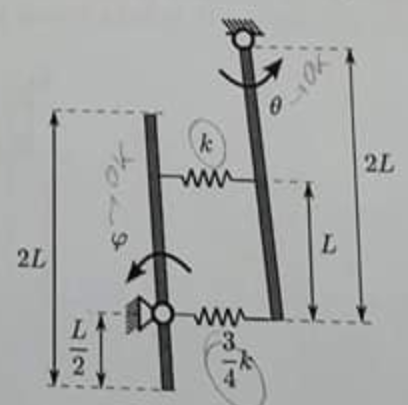
\includegraphics[width=.5\textwidth]{img/q2.png}
\end{center}
\begin{enumerate}
    \item Que vaut le champ magnétisant $H$ le long du cercle pointillé de rayon $R$, lorsque le courant $I = \SI{1}{\ampere}$ ?
    \item Que vaut alors le champ magnétique $B$ pour le matériau considéré ?
    \item Calculez l'inductance $L$ de ce dispositif.
\end{enumerate}

\begin{solution}
    \begin{enumerate}
        \item 
            Appelons $C$ le cercle de rayon $R$ en question. Par la loi d'Ampère
            \[ \oint_C \H \cdot \dif\vec{l} = I_\mathrm{tot}. \]
            Les spires étant bobinées régulièrement autour de ce cercle,
            le champ magnétisant est le même en tout point.
            Le courant total est la somme de chacun des courants traversant
            le contour fermé, c'est-à-dire $I_\mathrm{tot} = NI$.
            En remplaçant, on trouve
            \[ 2\pi R H = NI \Rightarrow H = \frac{NI}{2\pi R} \approx \SI{318.3}{\ampere\per\meter} \]
        \item 
            Puisqu'on considère le champ à l'intérieur du matériau, on multiplie le champ magnétisant par la perméabilité magnétique de ce matériau :
            \[ B = \pmb H = \vacpmb\relpmb H \approx \SI{.4}{\tesla} \]
        \item 
            Par définition, l'inductance du dispositif vaut
            \[ L \eqdef \frac{N\Phi}{I} \]
            où $\Phi$ est le flux magnétique d'une tranche arbitraire. Si $S$ est l'aire de cette tranche, on a
            \[ L = \frac{NBS}{I} = \frac{\pi NBr^2}{I} \approx \SI{.785}{\henry} \]
    \end{enumerate}
\end{solution}

\section{}
Une spire rectangulaire de dimensions $a$ fois $b$ est située dans le plan
$xOy$ à une distance $x$ d'un conducteur rectiligne infini placé le long de 
l'axe $Oy$ (voir figure ci-dessous). Le conducteur rectiligne est parcouru par
un courant $I$.

\begin{center}
    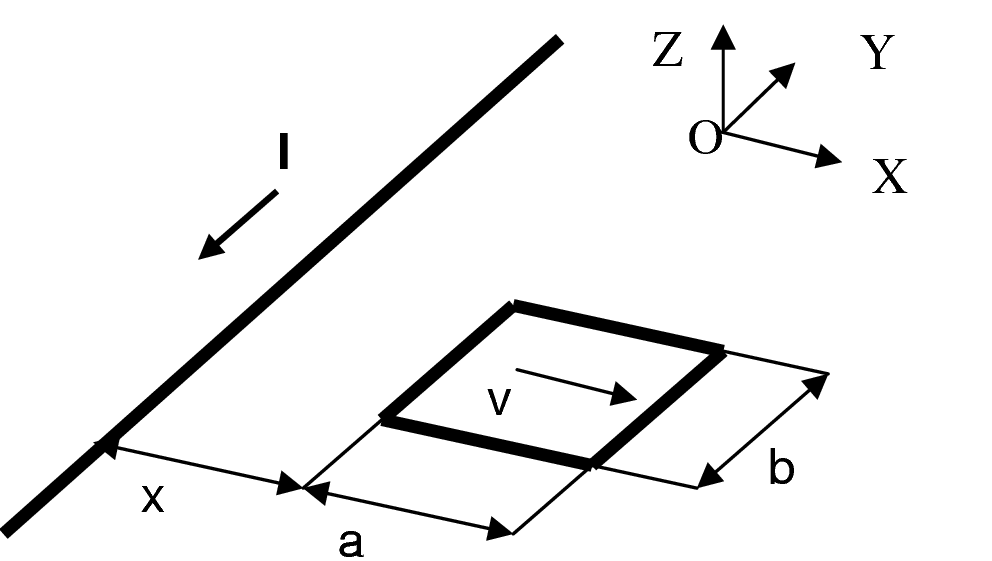
\includegraphics[width=.5\textwidth]{img/q3.png}
\end{center}

\begin{enumerate}
    \item Quelle est l'expression du flux magnétique intercepté par la spire
        rectangulaire produit par le courant $I$ (positif dans le sens
        indiqué) ?
    \item En appliquant sa définition, déduisez-en l'expression de l'inductance
        mutuelle entre la spire et le conducteur infini.
    \item Si maintenant, la spire glisse vers la droite suivant la relation
        $x(t) = x_0 + vt$, où $v$ est une constante positive (MRU), que vaut 
        l'expression de la force électromotrice $\EMF$ induite dans cette 
        spire pour un courant $I$ constant ?
    \item Que devient cette f.e.m. si, en plus du mouvement de
        translation précédent, le courant $I$ n'est plus constant mais
        sinusoïdal $I = I_0 \sin\omega t$ ?
\end{enumerate}

\begin{solution}
    \begin{enumerate}
        \item 
            Déterminons d'abord l'expression du champ magnétisant en fonction
            de la distance par rapport au fil. Soit un cercle $C$ de rayon $r$
            centré sur le fil et perpendiculaire à ce dernier. Par Ampère,
            \[ \oint_C \H\cdot\dl = I \]
            Puisque $\H$ est constant le long de la courbe et orienté 
            tangentiellement à celle-ci, l'équation devient
            \[ 2\pi r H = I \ \Rightarrow\  H(r) = \frac{I}{2\pi r} \]
            Par définition, le flux magnétique à travers la surface $S$ 
            s'exprime
            \[ \Phi = \int_S \B\cdot\dS \]
            $\B$ étant orienté selon $\uvz$ sur toute la surface et constant
            le long de $Oy$, on a
            \[ \Phi = \pmb_0 \int_S H \dif S
            = \pmb_0 b \int_x^{x+a} \frac{I}{2\pi r} \dif r \]
            Et en calculant l'intégrale, on obtient
            \[ \Phi = \frac{\pmb_0 bI}{2\pi} \ln\left(1 + \frac{a}{x} \right)\]
        \item 
            Par définition, l'inductance mutuelle entre le fil et la spire est
            le flux intercepté par la spire divisé par le courant dans le fil 
            qui induit ce flux. En équation, cela donne
            \[ M = \Phi / I = 
            \frac{\pmb_0 bI}{2\pi} \ln\left(1 + \frac{a}{x} \right) \]
        \item 
            L'expression du flux devient
            \[ \Phi(t) = \frac{\mu_0 bI}{2\pi} 
            \ln\left(1 + \frac{a}{x_0 + vt}\right) \]
            Et par la loi de Lenz-Faraday (on laisse les $x$ pour simplifier
            l'écriture),
            \[ \EMF = -\fdif{\Phi}{t} 
            = \frac{\pmb_0 abvI}{2\pi x(a+x)} \]
        \item Même procédé, on dérive l'expression du flux :
            \[ \EMF = \frac{\pmb_0 bI_0}{2\pi} 
                \left( \frac{av\sin\omega t}{x(a+x)} - 
            \omega \cos\omega t \ln\left(1 + \frac{a}{x} \right) \right) \]
    \end{enumerate}
\end{solution}

\end{document}
